%!TEX root = main_acm.tex

\section{Methodology}
\label{sec:meth}
In this section, we describe the datasets and the features we propose to extract from passively-collected BGP data for the purpose of identifying anycast routing. Using a reference dataset as {\it near}-ground-truth, we characterize the behavior of such BGP-related features in the wild. We then employ standard classification methods, decision tree and random forest, to train and evaluate the effectiveness of our approach for anycast detection using our proposed classification features. The repository including scripts and data used in our study is available at \cite{ccr_anycast}.

\subsection{Datasets}
\label{sec:data}
\subsubsection*{BGP Routing Information.} The datasets we used to detect and
characterize anycast prefixes are from the RouteViews project~\cite{Routeviews}
and RIPE's Routing Information Service (RIS)~\cite{RIPE_RIS}. 
In RouteViews and RIPE RIS, servers receive BGP information by peering with other BGP routers, often at large IXPs. We use CAIDA's BGPStream \cite{orsini2016bgpstream} to collect and process the data from RouteViews and RIPE RIS.

\subsubsection*{Anycast Dataset.} 
\label{sec:anycast_ground}
We use the anycast prefix list obtained through active measurements by Cicalese et al.~\cite{cicalese2015characterizing} as {\it near}-ground-truth, which provides a {\it conservative} estimation of Internet anycast usage.
The detection method in \cite{cicalese2015characterizing} is based on speed-of-light violations: if the latency measurements from multiple vantage points towards the same target exhibit geo-inconsistency, the target is  classified as anycast. They validated their method and scrutinized the dataset they make publicly available~\cite{DarioAnycastData} using ground-truth collected through protocol-specific techniques (e.g., DNS CHAOS requests or DPI over HTTP). 

However, we also notice that some prefixes strongly suggested as anycast by our method are not included in their dataset. We manually check and, through traceroute measurements, verify that most of them are indeed anycast prefixes. 
%Anycast prefixes missed by our method mostly belong to Microsoft, Google, CDNs and anycast-based DNS providers. The details are shown in \S\ref{sec:inaccu}. 

\begin{figure*}[th]
	\centerline{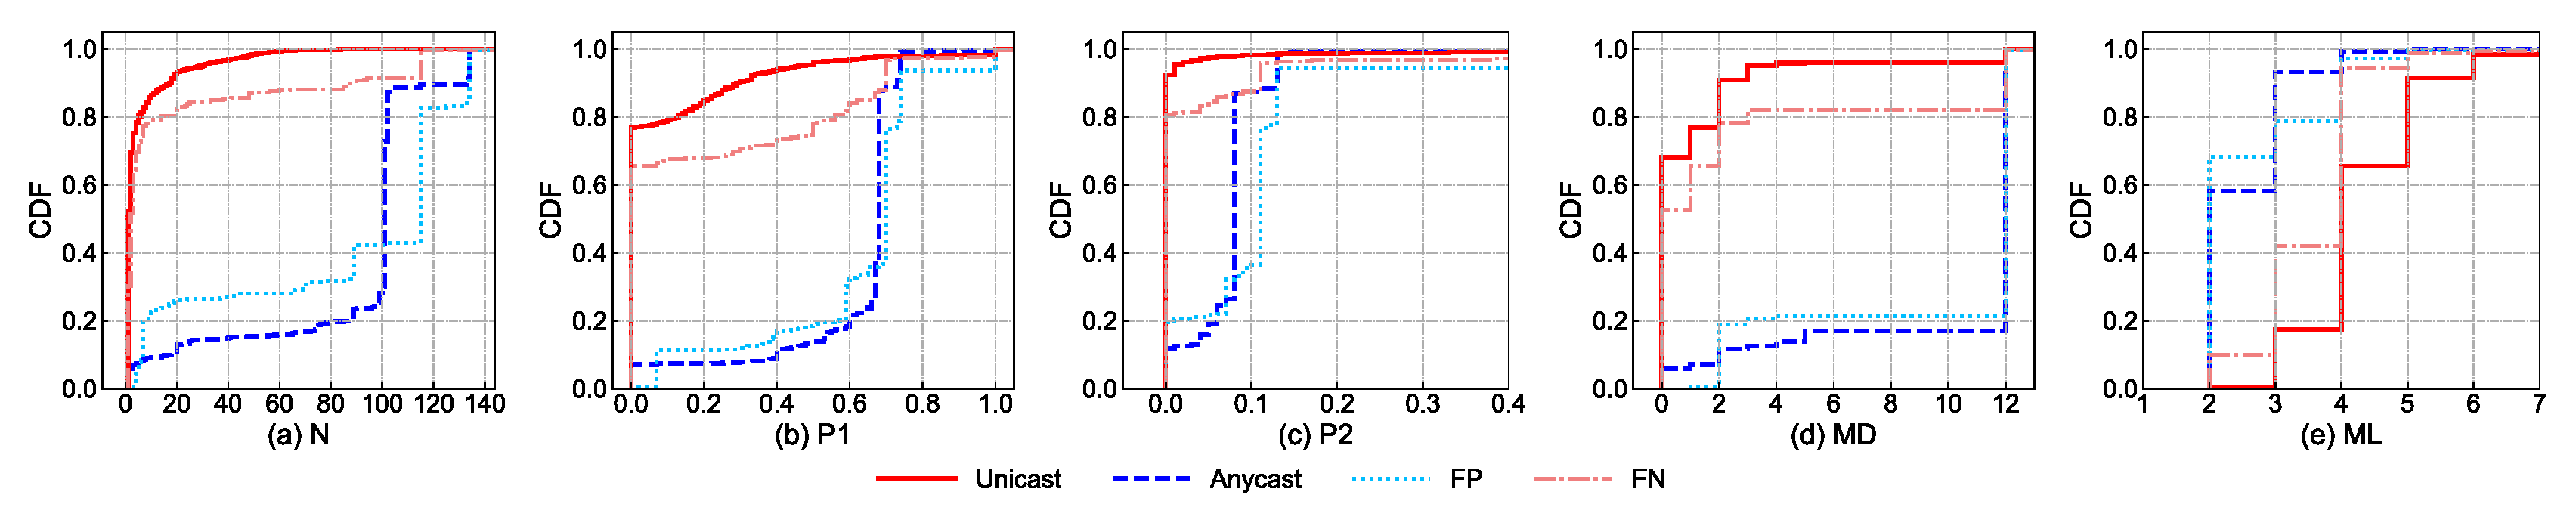
\includegraphics[scale=0.312]{fig/features.eps}}
	\vspace{3pt}
	\caption{ Distributions of the 5 classification features we propose for (1) anycast/unicast from the near-ground-truth dataset (\S\ref{feature}) and (2) False Positives/False Negatives from our passive classification (\S\ref{sec:inaccu})}
	\label{fig_FP_FN}
\end{figure*}

\subsection{BGP-related Features}

Due to the different deployment patterns between anycast and unicast, we leverage BGP routing information to characterize anycast prefixes. We propose and explore the following BGP-related features that could be used to identify anycast prefixes: as an anycast prefix is announced from multiple locations, some of its peer ASes should not be close to one another, both geographically and topologically.

\vspace{2pt}
\textbf{\texttt{N} - Number of upstream ASes:} We count the number of unique
\textit{upstream} ASes of each prefix. Given a prefix announced by $AS_{n}$, we
define \textit{upstream} ASes as the set of $AS_{n}$'s neighbor ASes that are
connected to $AS_{n}$ with either a customer-to-provider relationship (i.e.,
$AS_{n}$'s transit providers) or a peer-to-peer relationship, according to CAIDA's AS Relationships Dataset~\cite{as-rel}.

\textbf{\texttt{P1} - Percentage of upstream AS pairs whose distance is more than 1:}  We define the \textit{distance between two ASes} as the least number of AS hops between them in the observed paths.
For each prefix, we construct all the AS pairs between its upstream AS neighbors and label the number of AS pairs as $P$. We then identify the fraction of those AS pairs whose distance   is more than one, i.e., $P1=\ P_{dist>1}/ \ P$. 

\textbf{\texttt{P2} - Percentage of upstream-AS pairs whose distance is more than 2:} Similarly, P2 is defined as the fraction of those AS pairs with distance more than two, i.e., $P2=\ P_{dist>2}/ \ P$. Note that we propose P1 and P2 based on the assumption that the upstream ASes of an anycast prefix are more likely to be remote, both geographically and topologically.

\textbf{\texttt{MD} - Maximum distance between upstream ASes:} MD is the largest distance of two upstream ASes of a prefix. This variable tries to capture that upstream ASes for anycast prefixes are more spread out compared to unicast.

\textbf{\texttt{ML} - Maximum length of AS paths:} ML represents the length of
the longest AS path observed for a prefix. AS paths towards anycast prefixes
tend to be shorter, since they are announced from multiple locations. 

\subsection{Feature Validation}
\label{feature}

Given the features we proposed in \S3.2, we explore their potential for identifying anycast prefixes by analyzing their behavior with respect to prefixes labeled in the {\it near}-ground-truth dataset.  

\vspace{2pt}
\textbf{\texttt{N} }: Figure~\ref{fig_FP_FN}(a) shows the distributions of the number of upstream ASes, where we can see that the two classes of prefixes are clearly distinguishable from each other. Most anycast prefixes (90.2\%) have more than 17 upstream ASes, while 69.5\% of unicast prefixes only have one or two upstream ASes. This is consistent with the intuition that the routes towards an anycast prefix would be highly varied due to the geographically distributed deployment. 

\vspace{2pt}
\textbf{\texttt{P1}}: 
Figure~\ref{fig_FP_FN}(b) shows the distributions of P1. Obviously, P1 of
anycast prefixes is much larger than P1 of unicast prefixes. Specifically, P1 is
greater than 0.33 for 91.9\% of anycast prefixes,  and smaller than 0.07 for 78.1\% of unicast prefixes. A larger P1 for anycast prefixes implies that the upstream ASes are relatively far from one another because the upstream ASes of an anycast prefix are more geographically and topologically distributed. %\vspace{2pt}

\vspace{2pt}
\textbf{\texttt{P2}}: 
Similar to P1, from Figure~\ref{fig_FP_FN}(c), P2 is smaller than 1\% for 95.4\% of unicast prefixes but larger than 7\% for 73.7\% of anycast prefixes. 

\vspace{2pt}
\textbf{\texttt{MD}}:
Figure~\ref{fig_FP_FN}(d) shows the distributions of maximum distance between
upstream ASes for anycast and unicast prefixes. About 83.1\% of anycast's MD is
greater than 8 but 76.8\% of unicast prefixes' MD is smaller than 1. 

\vspace{2pt}
\textbf{\texttt{ML}}: 
Figure~\ref{fig_FP_FN}(e) shows the distributions of the longest AS paths for anycast and unicast prefixes. The ML of most anycast prefixes (93.3\%) is smaller than three hops, while only 18.3\% of ML for unicast prefixes are less than three. Anycast usually has a shorter maximum AS path than unicast, because anycast traffic is typically routed to the closest replica.

\subsection{The Classifier}

To further validate the effectiveness of identifying anycast from BGP paths, we
use a combination of our proposed features to build simple  (\textit{decision tree} and \textit{random forest}) classifiers and train them with the \textit{near}-ground-truth datasets by using the scikit-learn library~\cite{Scikit-learn} in Python. 

\vspace{2pt}
\textbf{The (\textit{near}-)Ground-Truth. }
The anycast dataset is described in \S\ref{sec:data}.  We use the monthly-refined datasets from 1/2017 to 6/2017 and retrieve the labeled anycast prefixes from a complete snapshot of BGP data by RIPE NCC and RouteViews on 6/1/2017. In total, we extract 3,907 anycast prefixes and label the remaining 728,010 prefixes as unicast.

\begin{table}[t]
\caption{Number of Prefixes in Classification}
\renewcommand{\arraystretch}{0.85}
\small
\begin{center}
\begin{tabular}{c c c c}
\toprule 
        & total & training & testing \\
\midrule 
Anycast & 3,907 & 2,609 & 1,298 \\
Unicast & 728,010 & 487,775 & 240,235  \\
total & 731,917 & 490,384  & 241,533 \\
\bottomrule
\end{tabular} 
\label{num_prefix_class}
\end{center}
\vspace{-3pt}
\end{table}

\begin{table}[t]
\caption{Evaluation of Classifiers}
\small
\renewcommand{\arraystretch}{0.85}
\begin{center}
\begin{tabular}{ c c c c}
\toprule 
        & precision & recall & f1-score \\
\midrule 
Decision Tree & 90.98\% & 89.45\% & 90.21\% \\
Random Forest & 93.94\% & 89.52\% & 91.68\%  \\
\bottomrule
\end{tabular} 
\label{res_dt_rf}
\end{center}
\vspace{-3pt}
\end{table}

\begin{table}[t]
\caption{Percentage of Mis-Classified Instances}
\small
\renewcommand{\arraystretch}{0.85}
\begin{center}
\begin{tabular}{c c c c }
\toprule 
        & Anycast & Unicast & Overall \\
\midrule 
Decision Tree & 10.55\% & 0.05\% & 0.10\% \\
Random Forest & 10.48\% & 0.03\% & 0.09\%  \\
\bottomrule
\end{tabular} 
\label{res_mis}
\end{center}
\vspace{-3pt}
\end{table}

\vspace{2pt}
\textbf{Evaluation of the Classifiers. }
We manually divide the labeled prefixes into exclusive training and testing sets, where 66\% of the dataset is used for training and the rest is used for testing. We use class-weights to handle unbalanced class sizes in the dataset.  Table~\ref{num_prefix_class} shows the detailed breakdown.
 
Table~\ref{res_dt_rf} lists the evaluation results of anycast classification using respectively a random forest and a decision tree classifier. Our results show that both classifiers can achieve high accuracy (more than 90\%). Table \ref{res_mis} lists the percentage of incorrectly classified instances. The fractions of incorrectly-labeled anycast prefixes in the two classifiers are 10.55\% and 10.48\%. For unicast, the misclassification rates are as low as 0.05\% and 0.03\%, respectively. 

